In this section we evaluate the performance of the proposed methodology in a variety of tasks. Results for 4 different experiments are reported. Experiment \ref{exp:1} compares the fitting accuracy of Dense Active Appearance Models (DAAMs) built using our methodology with respect to that of classic AAMs on the problems of non-rigid face and ear alignment in-the-wild. Experiment \ref{exp:2} investigates the impact that the Support Vector Shape representation has on the performance achieved by DAAMs on the the first experiment. Experiment \ref{exp:3} evaluates the effectiveness of the proposed methodology to build DAAMs of objects that are difficult to annotated with respect to a consistent set of landmarks, such as bottles and human bodies. Finally, experiment \ref{exp:4} serves as a qualitative demonstration of how the proposed pipeline can use be effectively used to generate novel modified instances of an object, e.g. caricatures, from simple hand drawn sketches.

\subsection{Shape representation and flow constraints}

\begin{figure}[t!]
\centering
\includegraphics[width=0.38\textwidth]{resources/Fig_Alignment/svs_experiment}
\caption{CED over 68 landmarks on the LFPW database.}
\label{fig:face_ced}
\end{figure}

\begin{table}[t]
\small
\centering
\begin{tabular}{|l|c|c|c|}
\hline
\emph{Method}         & \emph{mean $\pm$ std} & \emph{median} & $\leq 0.05$\\
\hline
Initialization        & $\pm$ & & \%\\
\hline
SVS representation    & $\pm$ & & \%\\
Binary representation & $\pm$ & & \%\\
\hline
Constraint Flow       & $\pm$ & & \%\\
Unconstrained Flow    & $\pm$ & & \%\\
\hline
\end{tabular}
\caption{Fitting statistics on the LFPW database.}
\label{tab:face_statistics}
\end{table}

\begin{figure}[h!]
    \centering
    \begin{subfigure}[b]{0.45\textwidth}
        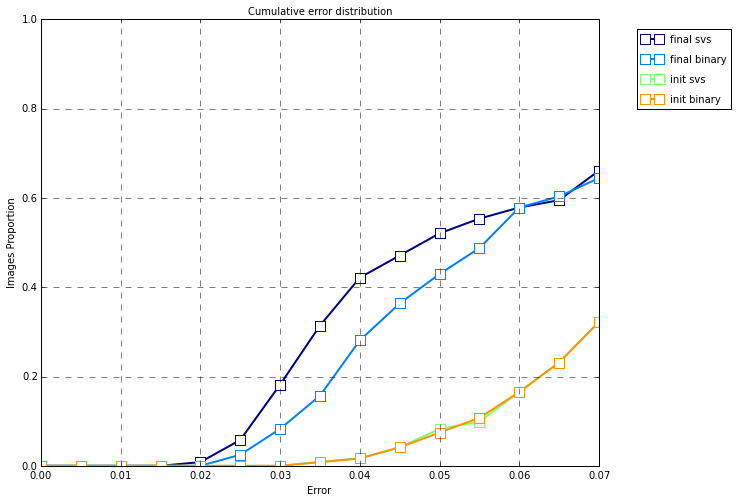
\includegraphics[width=\textwidth]{resources/Fig_SVS/faces_svs_binary_gaussian}
        \caption{AAM Principle Components Contribution}
    \end{subfigure}
    \hfill
    \begin{subfigure}[b]{0.2\textwidth}
            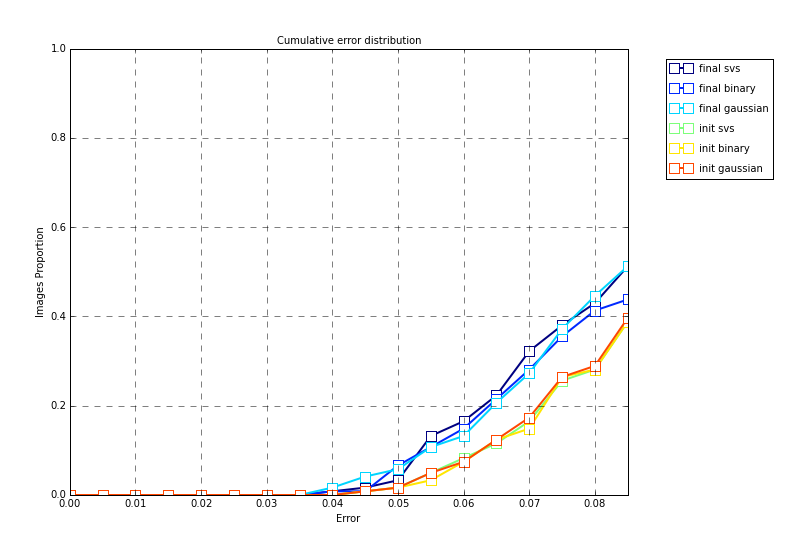
\includegraphics[width=\textwidth]{resources/Fig_SVS/ears_svs_binary_gaussian}
        % \caption{Shape Flow Principle Components Contribution}
    \end{subfigure}
    \\
    \begin{subfigure}[b]{0.2\textwidth}
            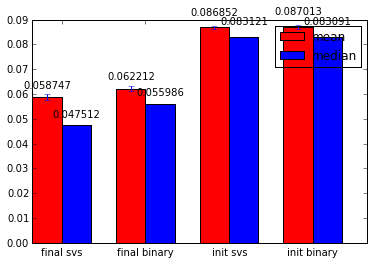
\includegraphics[width=\textwidth]{resources/Fig_SVS/faces_svs_binary_gaussian_statistics}
        % \caption{AAM Principle Components Contribution}
    \end{subfigure}
    \hfill
    \begin{subfigure}[b]{0.2\textwidth}
            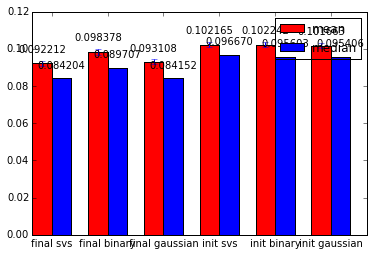
\includegraphics[width=\textwidth]{resources/Fig_SVS/ears_svs_binary_gaussian_statistics}
        % \caption{Shape Flow Principle Components Contribution}
    \end{subfigure}
    \caption{Principle Components Contribution}
\end{figure}



\subsection{Non-rigid object alignment in-the-wild}
\label{exp:1}

\subsubsection{Face alignment}

This experiment compares the fitting accuracy of our DAAMs and classic AAMs. For this experiment, both models were built using the 811 training images of the Labelled Faces Parts in-the-Wild (LFPW) \cite{} database and corresponding 68 point annotations provided by the iBUG group \footnote{\label{ibug_300}\url{http://ibug.doc.ic.ac.uk/resources/300-W/}}. Classic AAMs were built using the standard procedure described in \cite{} using piece-wise affine as their motion model. Our DAAMs were built using the methodology described on the main part of the paper. Notice that we modified the previous 68 point annotations of all images by adding and removing $\pm$5 to and from the that were not or subtracted $\approx$ 

Results for this experiment are reported over the 224 test images of the LFPW cite{} database. 66
points ground truth landmark annotations were provided by
the iBUG group8
. All methods were initialized by perturbing
the ground truth scale and translation parameters with
Gaussian noise (rotations were not considered) and applying
the resulting transformation to mean of the shape model.
(Notice that this procedure produces initializations that are
considerably more challenging than those reported in the recent
AAM literature [32, 33]). The Cumulative Error Distributions
(CED) for this experiment is shown in Figures 1
and 2. Figures 3 and 4 shows the evolution of the mean
normalized point-to-point error as a function of the number
of iterations run by each algorithm

\begin{figure}[t!]
\centering
\includegraphics[width=0.38\textwidth]{resources/Fig_Alignment/face_experiment}
\caption{CED over 68 landmarks on the LFPW database.}
\label{fig:face_ced}
\end{figure}

\begin{table}[t]
\small
\centering
\begin{tabular}{|l|c|c|c|}
\hline
\emph{Method}   & \emph{mean $\pm$ std} & \emph{median} & $\leq 0.05$\\
\hline
Initialization  & $\pm$ & & \%\\
\hline
INT - dAAM      & $\pm$ & & \%\\
INT - AAM       & $\pm$ & & \%\\
HOG - dAAM      & $\pm$ & & \%\\
HOG - AAM       & $\pm$ & & \%\\
\hline
\end{tabular}
\caption{Fitting statistics on the LFPW database.}
\label{tab:face_statistics}
\end{table}


%\begin{figure}[h!]
%    \centering
%    \begin{subfigure}[b]{0.2\textwidth}
%            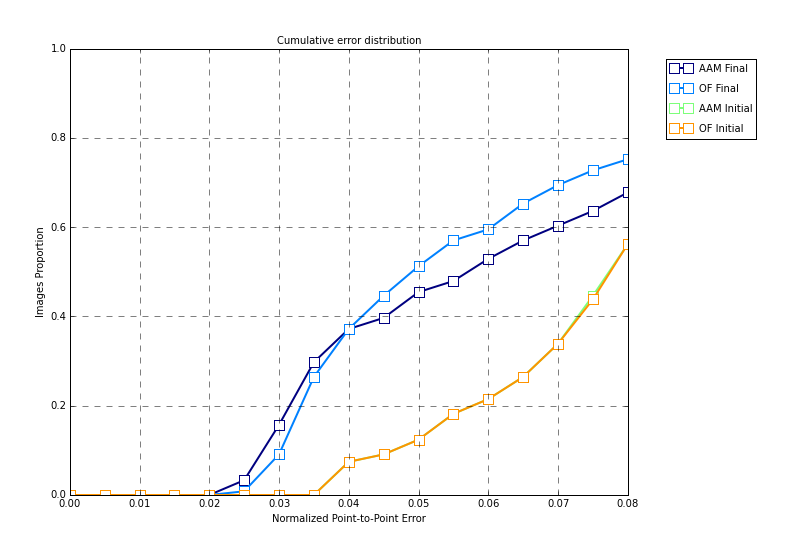
\includegraphics[width=\textwidth]{resources/Fig_Alignment/face_intensity}
%        % \caption{AAM Principle Components Contribution}
%    \end{subfigure}
%    \hfill
%    \begin{subfigure}[b]{0.2\textwidth}
%            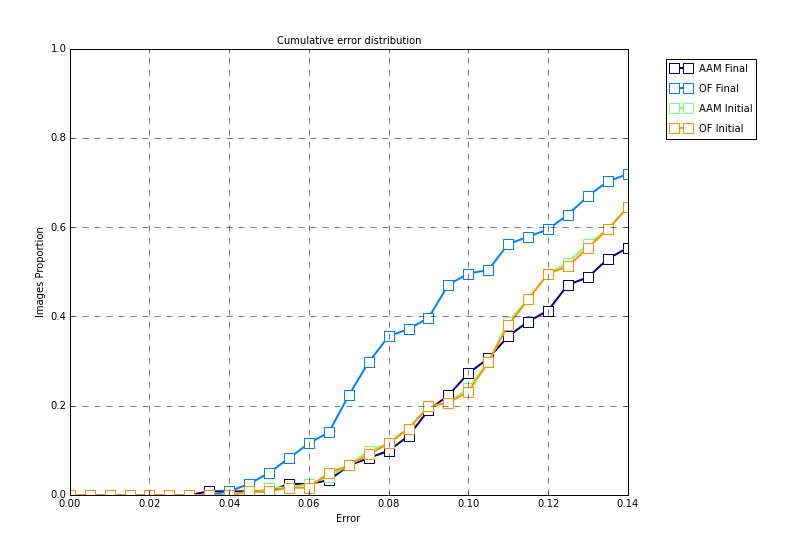
\includegraphics[width=\textwidth]{resources/Fig_Alignment/ear_intensity}
%        % \caption{Shape Flow Principle Components Contribution}
%    \end{subfigure}
%    \\
%    \begin{subfigure}[b]{0.2\textwidth}
%            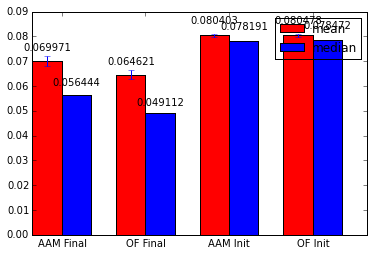
\includegraphics[width=\textwidth]{resources/Fig_Alignment/face_intensity_statistics}
%        % \caption{AAM Principle Components Contribution}
%    \end{subfigure}
%    \hfill
%    \begin{subfigure}[b]{0.2\textwidth}
%            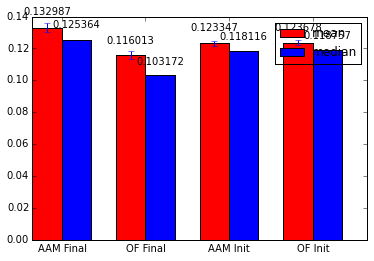
\includegraphics[width=\textwidth]{resources/Fig_Alignment/ear_intensity_statistics}
%        % \caption{Shape Flow Principle Components Contribution}
%    \end{subfigure}
%    \caption{CED Plot and Statistics of Comparison with Classic AAM}
%\end{figure}

\subsubsection{Ear alignment}


\subsubsection{Objects with loosely define landmarks}


\subsection{DAAMs without consistent annotations}
\label{exp:3}

\subsection{Object generation from sketches}
\label{exp:4}

\begin{figure}[h!]
    \centering
    \begin{subfigure}[b]{0.1\textwidth}
            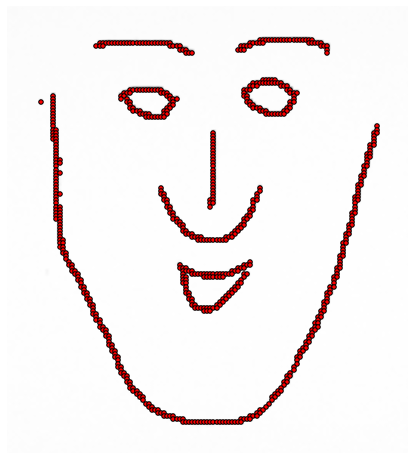
\includegraphics[width=\textwidth]{resources/Fig_Draw/test_01}
    \end{subfigure}
    \hfill
    \begin{subfigure}[b]{0.12\textwidth}
            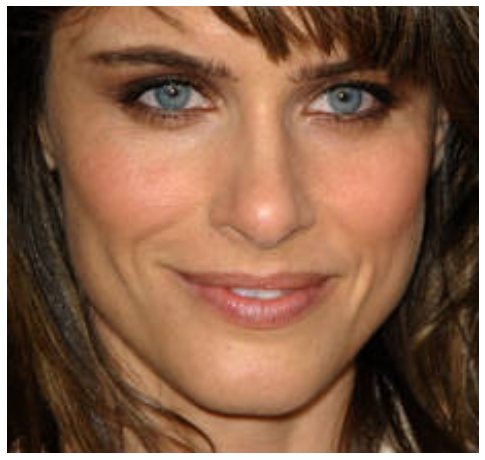
\includegraphics[width=\textwidth]{resources/Fig_Draw/test_01_base}
    \end{subfigure}
   	\hfill
    \begin{subfigure}[b]{0.1\textwidth}
            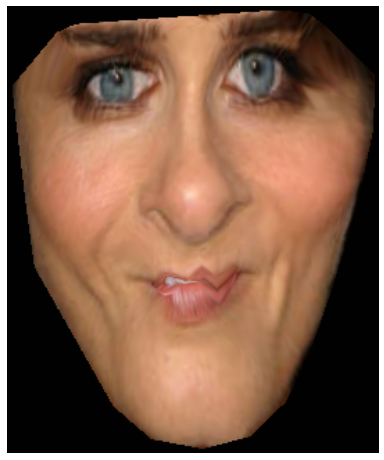
\includegraphics[width=\textwidth]{resources/Fig_Draw/test_01_aam}
    \end{subfigure}
    \hfill
    \begin{subfigure}[b]{0.1\textwidth}
            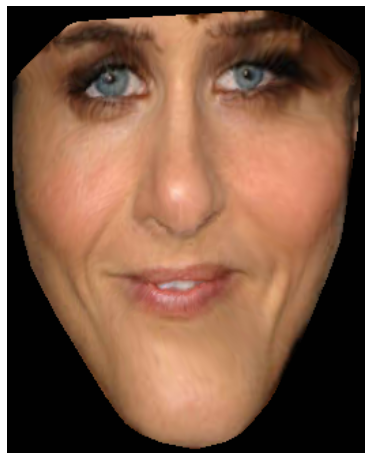
\includegraphics[width=\textwidth]{resources/Fig_Draw/test_01_of}
    \end{subfigure}
    \\
    \begin{subfigure}[b]{0.1\textwidth}
            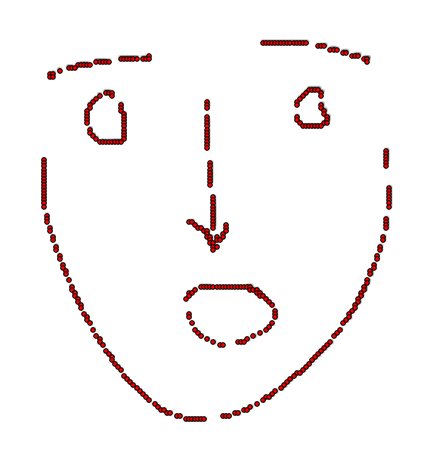
\includegraphics[width=\textwidth]{resources/Fig_Draw/test_02}
    \end{subfigure}
    \hfill
    \begin{subfigure}[b]{0.12\textwidth}
            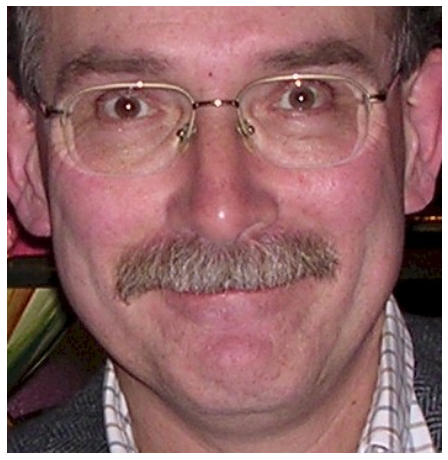
\includegraphics[width=\textwidth]{resources/Fig_Draw/test_02_base}
    \end{subfigure}
   	\hfill
    \begin{subfigure}[b]{0.1\textwidth}
            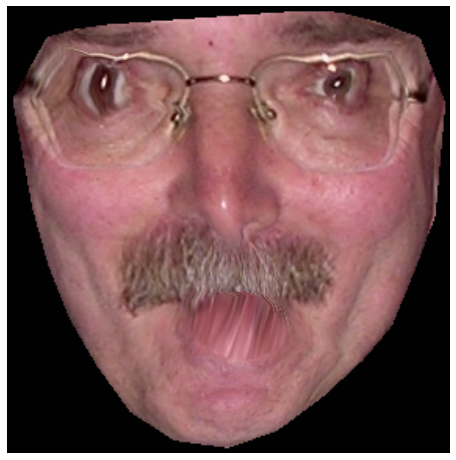
\includegraphics[width=\textwidth]{resources/Fig_Draw/test_02_aam}
    \end{subfigure}
    \hfill
    \begin{subfigure}[b]{0.1\textwidth}
            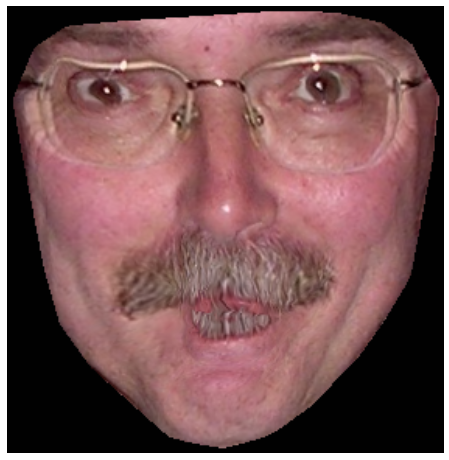
\includegraphics[width=\textwidth]{resources/Fig_Draw/test_02_of}
    \end{subfigure}
    \\
    \begin{subfigure}[b]{0.1\textwidth}
            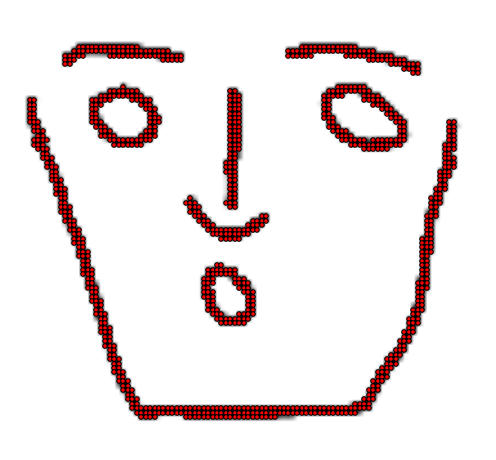
\includegraphics[width=\textwidth]{resources/Fig_Draw/test_03}
    \end{subfigure}
    \hfill
    \begin{subfigure}[b]{0.12\textwidth}
            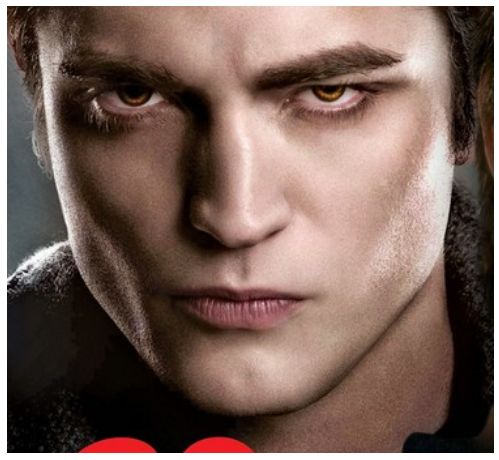
\includegraphics[width=\textwidth]{resources/Fig_Draw/test_03_base}
    \end{subfigure}
   	\hfill
    \begin{subfigure}[b]{0.1\textwidth}
            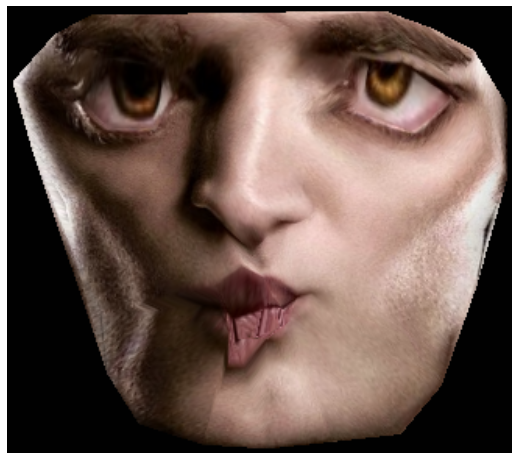
\includegraphics[width=\textwidth]{resources/Fig_Draw/test_03_aam}
    \end{subfigure}
    \hfill
    \begin{subfigure}[b]{0.1\textwidth}
            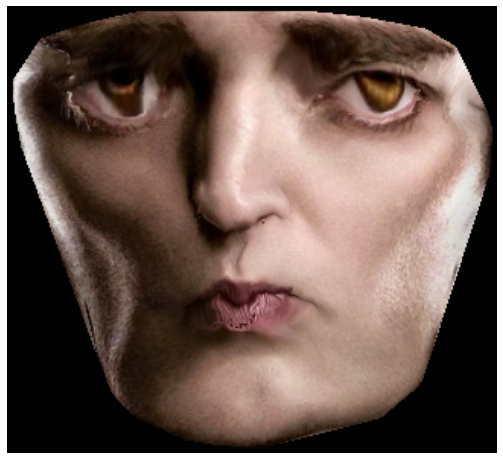
\includegraphics[width=\textwidth]{resources/Fig_Draw/test_03_of}
    \end{subfigure}
    \\
    \begin{subfigure}[b]{0.1\textwidth}
            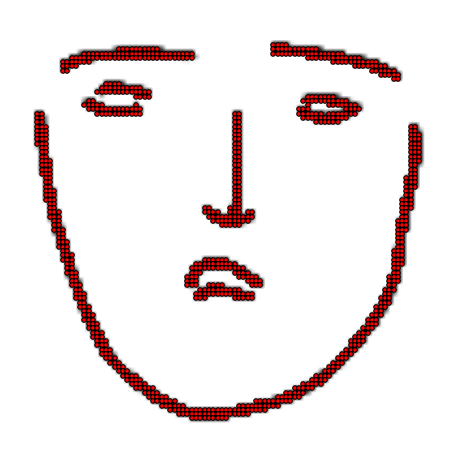
\includegraphics[width=\textwidth]{resources/Fig_Draw/test_04}
    \end{subfigure}
    \hfill
    \begin{subfigure}[b]{0.12\textwidth}
            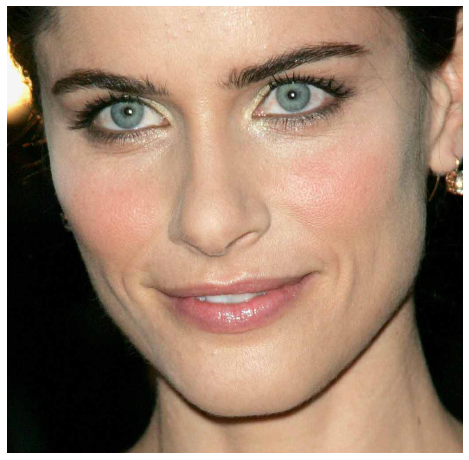
\includegraphics[width=\textwidth]{resources/Fig_Draw/test_04_base}
    \end{subfigure}
   	\hfill
    \begin{subfigure}[b]{0.1\textwidth}
            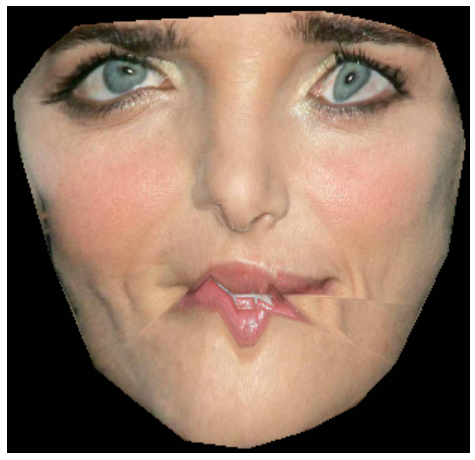
\includegraphics[width=\textwidth]{resources/Fig_Draw/test_04_aam}
    \end{subfigure}
    \hfill
    \begin{subfigure}[b]{0.1\textwidth}
            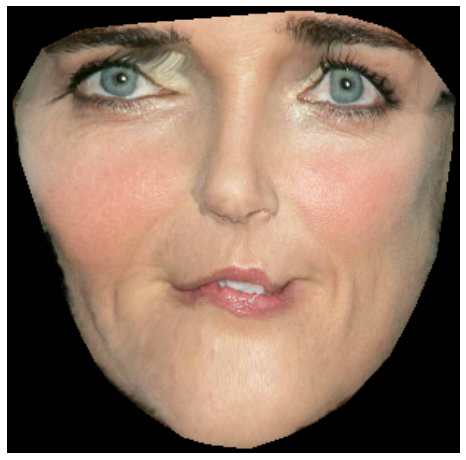
\includegraphics[width=\textwidth]{resources/Fig_Draw/test_04_of}
    \end{subfigure}
    \caption{Figure}
    \label{fig:draw}
\end{figure}

\clearpage